\documentclass[tikz, border=10pt]{standalone}

\usetikzlibrary{arrows}

\begin{document}
	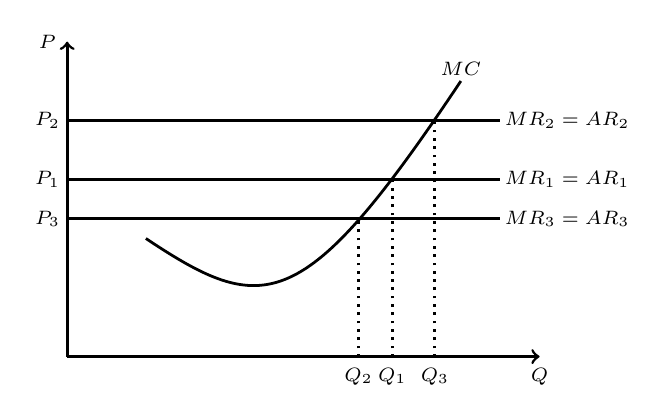
\begin{tikzpicture}[line width=1pt]
	
		\draw[->] (0, 0) -- (6, 0); % Горизонтальная линия
		\draw[->] (0, 0) -- (0, 4); % Вертикальная линия
	
		\draw (1, 1.5) .. controls (2.5, 0.5) and (3, 0.5) .. (5, 3.5); % Кривая AS
		
		\draw (0, 1.75) -- (5.5, 1.75);
		\draw (0, 2.25) -- (5.5, 2.25);
		\draw (0, 3) -- (5.5, 3);
		
		\draw[dotted] (3.7, 0) -- (3.7, 1.75);
		\draw[dotted] (4.13, 0) -- (4.13, 2.25);
		\draw[dotted] (4.67, 0) -- (4.67, 3);

	\begin{scriptsize}
		\draw (-0.25, 4) node {$P$};
		\draw (6, -0.25) node {$Q$};
		\draw (5, 3.65) node {$MC$};
		
		\draw (-0.25, 1.75) node {$P_3$};
		\draw (-0.25, 2.25) node {$P_1$};
		\draw (-0.25, 3) node {$P_2$};
		
		\draw (6.35, 1.75) node {$MR_3=AR_3$};
		\draw (6.35, 2.25) node {$MR_1=AR_1$};
		\draw (6.35, 3) node {$MR_2=AR_2$};
		
		\draw (3.7, -0.25) node {$Q_2$};
		\draw (4.13, -0.25) node {$Q_1$};
		\draw (4.67, -0.25) node {$Q_3$};
	\end{scriptsize}
	\end{tikzpicture}
\end{document}